\documentclass[11pt, a4paper]{article}
\usepackage[italian]{babel} % Imposta l'italiano come lingua del documento
% Rimuovi il pacchetto fontspec e il comando \setmainfont{Open Sans}
% Il pacchetto fontspec e \setmainfont funzionano solo con XeLaTeX o LuaLaTeX e possono causare la perdita del corsivo con pdflatex.
% Il corsivo (\textit{}) funziona correttamente con i font standard di LaTeX (Computer Modern o lmodern).

% Pacchetti per una migliore tipografia
\usepackage[T1]{fontenc}
\usepackage[utf8]{inputenc}
\usepackage{lmodern}
\usepackage{microtype}
\usepackage{float}

% Pacchetti per l'aspetto della pagina
\usepackage{geometry}
\geometry{a4paper, margin=2.5cm}

\usepackage{setspace}
\onehalfspacing

% Pacchetti per titoli e intestazioni personalizzate
\usepackage{titlesec}
{\normalfont\Large\bfseries}
\titlespacing*{\section}{0pt}{1.5ex plus .2ex minus .2ex}{1ex plus .2ex}


% Imposta la didascalia delle figure più piccola e senza "Figura N"
\usepackage{caption}
\captionsetup[figure]{
    font=small,          % Didascalia più piccola
    labelformat=empty    % Nessuna etichetta "Figura N"
}
{\normalfont\Large\bfseries}

\titleformat{\subsection}
{\normalfont\large\bfseries\itshape}
{\thesubsection}{1em}{}

\usepackage{fancyhdr}
\pagestyle{fancy}
\fancyhf{}
\fancyhead[L]{\nouppercase{\leftmark}} % Intestazione a sinistra per tutte le pagine
\fancyhead[R]{\thepage}                % Numero di pagina a destra per tutte le pagine
\renewcommand{\headrulewidth}{0.5pt}
\renewcommand{\footrulewidth}{0pt}

% Pacchetti per elementi visivi (opzionale)
\usepackage{graphicx}
\usepackage{xcolor}
\usepackage{svg}

\fancyfoot[L]{\textit{Simone Arena}}
\fancyfoot[C]{}
\fancyfoot[R]{\textit{Simone Home Hub}}

% Ipercollegamenti (opzionale)
\usepackage{hyperref}
\hypersetup{
    colorlinks=true,
    linkcolor=blue,
    citecolor=blue,
    urlcolor=blue
}

% Pacchetti per elementi visivi (opzionale)
\usepackage{graphicx}             % Inserimento di immagini
\usepackage{xcolor}               % Gestione dei colori

% Ipercollegamenti (opzionale)
\usepackage{hyperref}
\hypersetup{
    colorlinks=true,
    linkcolor=blue,
    citecolor=blue,
    urlcolor=blue
}

\usepackage{etoolbox}
\AtBeginEnvironment{verbatim}{%
    \small
    \renewcommand{\baselinestretch}{0.75}%
    \ttfamily
}

% \usepackage{fontspec}
% \setmainfont{Open Sans}


\title{Simone Home Hub}
\author{Simone Arena}
\date{}

\begin{document}

\color{black}

\maketitle

\begin{center}
    5CI\\
    A.S. 2024-2025
\end{center}

\begin{figure}[h!]
    \centering
    \includegraphics[width=0.2\textwidth]{media/Home_Assistant_logo_(2023).svg}
    \hspace{1cm} % Spazio tra le immagini
    \includegraphics[width=0.2\textwidth]{media/esphome-logo.jpeg}
    \label{fig:logos}
\end{figure}

\newpage

\tableofcontents

\newpage

\begin{figure}[h!]
    \centering
    \includegraphics[width=1\textwidth]{media/iot-banner.jpg}
    \label{fig:iot-banner}
\end{figure}
\section{Introduzione}
Il presente progetto si inserisce nel dinamico 
e in continua evoluzione panorama dell'IoT, l'Internet delle cose
 e dell'analisi dei Big Data, ambiti dinamici e continua evoluzione. 
L'IoT rappresenta una fitta rete di dispositivi 
fisici interconnessi, capaci di raccogliere e 
scambiare dati in tempo reale. Questa mole crescente 
di informazioni, definita come Big Data, offre opportunità 
senza precedenti per comprendere e ottimizzare il nostro ambiente, 
in particolare all'interno delle nostre abitazioni. 
In questo contesto, esploreremo le potenzialità di una 
piattaforma open-source di home automation come \textit{Home Assistant}, 
focalizzandoci su come essa possa agire da fulcro per l'integrazione 
di diversi dispositivi intelligenti e per la gestione dei dati generati, 
aprendo la strada a soluzioni innovative per una casa più efficiente, 
sicura e personalizzata.

\subsection*{Metanote sul documento}
Questo documento è stato redatto in LaTeX (pronuncia: \textit{latec}), un linguaggio di markup
(come lo è l'HTML) per la scrittura di documenti scientifici e tecnici.
LaTeX è particolarmente utile per la creazione di documenti complessi, come tesi, articoli scientifici e relazioni tecniche, 
grazie alla sua capacità di gestire formule matematiche, indici, bibliografie e riferimenti incrociati in modo efficiente.
Grazie alla sua sintassi, LaTeX permette di separare il contenuto dalla formattazione permettendo
agli autori di concentrarsi esclusivamente sul testo, senza preoccuparsi dell'aspetto final del documento.
L'utilizzo di LaTeX è liberamente diffuso in ambito accademico e scientifico.

\begin{figure}[H]

    \centering
    \includegraphics[width=0.4\textwidth]{media/LaTeX_logo.svg}
    \caption{Logo di LaTeX}
    \label{fig:latex-logo}

\end{figure}

\subsection{Obiettivi}
L'obiettivo di questo progetto è l'automazione domotica della mia abitazione.
Dato che è in arrivo l'estate, e insieme a mio padre, come tutti gli anni, ho allestito
l'orto, quest'anno l'obiettivo è quello di cominciare questo progetto domotico
proprio dall'automazione dell'orto stesso.
Al momento, il mio orto è munito di irrigazione a goccia, con dei tubi forati
che corrono lungo le file di pomodori, peperoni, insalata, ravanello e zucchine.
I tubi forati sono collegati a una pompa per liquidi, che pesca l'acqua dal nostro
pozzo. Ogni giorno, quindi, è necessario andare a controllare lo stato di irrigazione
delle piante, accendere manualmente la pompa del pozzo quando necessario e successivamente
spegnerla quando il terreno sarà sufficientemente umido.
Tutti questi passaggi potrebbero essere opportunamente automatizzati, sollevando me,
mio padre e mio zio da un lavoro ripetitivo e pesante, considerato il clima afoso
che si verifica in molti giorni della stagione estiva.
Una soluzione soddisfacente dovrebbe consistere in un'infrastuttura accessibile tramite web
che preveda:
\begin{itemize}
    \item Il monitoraggio del livello di umidità del suolo;
    \item L'accensione automatizzata o manuale tramite web app della pompa del pozzo;
    \item La possibilità di bypassare l'irrigazione automatica e controllare la pompa
            tramite pulsanti fisici presenti nell'orto oltre che da remoto.
\end{itemize}
Un'ulteriore funzionlità che sarebbe interessante ed utile implementare sarebbe l'installazione
di una telecarmera all'interno del pollaio che permetta di controllare remotamente lo stato delle galline
e il numero di uova deposte.
Tutto ciò deve essere accessibile da smartphone e da computer, per permettere la massima
comodità.
Come infrastuttura per permettere la realizzazione del progetto è stata scelta Home Assistant.

\subsection{Home Assistant}

\subsubsection{Cos'è Home Assistant}
\textit{Home Assistant} è una piattaforma di automazione domestica. È gratis e open-source, e
rappresenta un'alternativa, completamente locale, a servizi come HomeBridge e SmartThings che
elaborano i dati presso i loro server remoti.

\subsubsection{Perchè Home Assistant}
Home Assistant rende possibile l'automazione domestica senza la necessità di un cloud,
quindi senza dipendere dall'infrastuttura internet, da server remoti o da servizi esterni.
Questo rende l'esperienza utente più fluida e l'operabilità piu affidabile.
Un sistema basato su Home Assistant è di sua natura un sistema DIY (Do It Yourself), ossia "fai da te", dato che viene affidata
all'utente la programmazione dei microcontrollori, la creazione dell'elettronica che orbita
intorno ad essi e il setup del server stesso. La sua vasta compatibilità
con i dispositivi è dovuta proprio al fatto che ogni sensore o microcontrollore
deve essere configurato e programmato individualmente. Ciò permette numerose possibilità di
personalizzazione: ogni sistema può essere adattato alle esigenze specifiche dell'utente.
In sintesi, utlizzare Home Assistant in questo progetto:
\begin{itemize}
    \item Ha reso possibile la creazione di un sistema di automazione domestica completamente artigianale,
        progettato e sviluppato da me;
    \item Permette di creare un sistema completamente locale, nel quale dati non fuoriescono dalla mia rete;
    \item Permette di gestire i sensori e gli attuatori a distanza con interfaccia web in modo semplice e intuitivo;
    \item Permette di integrare facilmente i microcontrollori e i sensori che saranno utilizzati in questo progetto;
\end{itemize}

\subsubsection{Perché preferire HAss alle soluzioni cloud-based}
La grande maggioranza dei dispositivi smart è progettata per essere utilizzata basandosi su
un'infrastuttura basata sul web, che spesso rende più facile e immediato il setup iniziale per gli utenti,
ma anche più capillare il controllo dei dati da parte dei produttori, come la raccolta e l'analisi dei dati
raccolti dal sistema domotico. Questo è un aspetto che non deve essere sottovalutato, in quanto
l'analisi dei dati è una pratica sempre più diffusa, che sta permettendo alle case produttrici di
ottimizzare i propri prodotti, ma se non gestita correttamente, può portare a violazioni della privacy
e alla diffusione di dati sensibili.

\subsection{ESPHome}

Per poter integrare all'interno di Home Assistant i microcontrollori che saranno utilizzati sarà necessaria
l'implementazione di un firmware che permetta la comunicazione tra i microcontrollori e il server.
Per questo, è stato scelto di utilizzare \textit{ESPHome}.

\begin{figure}[h!]
    \centering
    \includegraphics[width=0.4\textwidth]{media/mio-esp-32.jpg}
    \caption{Foto di un microcontrollore basato su ESP32, montato su opportuna dev board.}
    \label{fig:esphome-dashboard}
\end{figure}

\subsubsection{Cos'è ESPHome}
\href{https://esphome.io}{\textit{ESPHome}} è un 
framework\footnote{Un framework è un insieme di strumenti, librerie e regole che facilita 
lo sviluppo di applicazioni, fornendo una struttura di base su cui costruire.} 
\textbf{open-source} che permette di 
creare firmware personalizzati per dispositivi basati su ESP8266, ESP32 e RP2040,
che sono ampiamente utilizzati in progetti di automazione domestica e IoT grazie alla loro versatilità e facilità d'uso.



\subsubsection{Perché ESPHome}
\begin{itemize}
    \item In questo progetto verranno utilizzati dispositivi basati su ESP8266 e ESP32;
    \item ESPHome semplifica la configurazione e la programmazione di questi dispositivi, 
    consentendo agli utenti di definire il comportamento del dispositivo attraverso un file di configurazione \textit{YAML},
    che verrà descritto nel paragrafo 
    \ref{sec:yaml-configurazione} (vedi \hyperref[sec:yaml-configurazione]{Configurazione tramite YAML}).
    In questo file, gli utenti possono specificare le funzionalità desiderate, come sensori, attuatori e altre componenti hardware. 
    Una volta configurato, ESPHome genera automaticamente il firmware necessario per il microcontrollore, che può essere caricato
    direttamente sul dispositivo in modalità \textit{OTA}, ovvero \textit{Over The Air}, cioè senza la necessità di collegare 
    fisicamente il dispositivo ad una macchina quale il computer o il server;
    \item ESPHome consente di risparmiare tempo e fatica nella scrittura del codice, rendendo 
            l'automazione domestica più accessibile anche a chi non ha esperienza di programmazione;
    \item ESPHome offre un'integrazione fluida con Home Assistant, consentendo agli utenti di 
            monitorare e controllare i dispositivi direttamente dalla dashboard.

\end{itemize}

\section{Sviluppo del progetto}

\subsection{Setup del server}
Per l'hosting di Home Assistant di questo progetto è stato scelto un server dedicato.
Il server in questione non è altro che un computer da ufficio datato e ormai in disuso, basato su
piattaforma x86\footnote{x86 è una famiglia di architetture di processori 
compatibili con i PC, sviluppata originariamente da Intel. Indica comunemente 
i computer basati su processori Intel o compatibili, a differenza di altre architetture come ARM.}.
In questo caso Home Assistant sarà installato come un vero sistema operativo, che verrà esclusivamente
gestito dal computer dedicato.

\begin{figure}
    
    \centering
    \includegraphics[width=0.4\textwidth]{media/server-home-assistant.jpg}
    \caption{Foto del server dedicato all'hosting di Home Assistant}
    \label{fig:server-dedicato}

\end{figure}

\subsubsection{Preparazione della macchina}
È fondamentale che la macchina dedicata sia in buone condizioni, che non presenti problemi hardware e che
i componenti al suo interno siano orientati al risparmio energetico. Essendo un computer destinato
a rimanere acceso 24 ore su 24, è importante che al suo interno sia munito di adeguati sistemi di raffreddamento.

\subsubsection{Scelta dell'hardware}
La scelta dell'hardware è fondamentale per garantire prestazioni ottimali e un funzionamento affidabile del sistema.
Per l'installazione del sistema operativo è richiesto un computer con almeno 2 GB di RAM e 32 GB di spazio di archiviazione.
Home Assistant OS può essere installato sia su \textit{SBC} (Single Board Computer), come un \textit{Raspberry Pi\footnote{
    Raspberry Pi è un single-board computer sviluppato dalla Raspberry Pi Foundation,
    nato con l'obiettivo di promuovere l'insegnamento dell'informatica nelle scuole e nei paesi in via di sviluppo.
    È caratterizzato da dimensioni estremamente compatte, basso consumo energetico e un costo contenuto,
    rendendolo ideale per progetti di automazione, domotica, robotica e prototipazione elettronica.
}}, 
che su una comune macchina x86.
Nella scelta del supporto di memoria, è preferibile optare per un'unità a stato solido (SSD) 
piuttosto che un disco rigido tradizionale (HDD),
in quanto, oltre alle prestazioni nettamente superiori, gli SSD non prevedono parti meccaniche in movimento e non sono quindi
soggetti a usura meccanica.

\subsubsection{Installazione del sistema operativo}
In questo caso, il sistema operativo scelto è \textit{Home Assistant Operating System}, che è una distribuzione Linux
ottimizzata per eseguire Home Assistant, che non prevede un'interfaccia grafica, ma è gestita tramite un'interfaccia web.
Questo sistema operativo è progettato per essere installato su hardware dedicato, come un Raspberry Pi o un server x86, 
e offre un'installazione semplificata e una gestione centralizzata dei dispositivi e delle automazioni.
L'installazione di Home Assistant OS è un processo relativamente semplice:
\begin{enumerate}
    \item Scaricare l'immagine del sistema operativo dal \href{https://www.home-assistant.io/installation/}{sito ufficiale} 
    di Home Assistant;
    \item Creare un'unità USB avviabile utilizzando un software come \href{https://etcher.balena.io}{\textit{Balena Etcher}} o 
        \href{https://rufus.ie/it/}{Rufus};
    \item Avviare il computer dal supporto USB e seguire le istruzioni per completare l'installazione.
    \item Una volta completata l'installazione, il sistema si riavvierà e Home Assistant sarà accessibile 
            all'interno della stessa rete locale tramite browser web all'indirizzo IP del server.
\end{enumerate}
Solamente durante questo processo sarà necessario un monitor e una tastiera, che serviranno per interagire con l'interfaccia
a testo per la primissima configurazione.

\subsubsection{Posizionamento del server}
Una volta completata l'installazione, il server può essere posizionato in un luogo strategico all'interno della casa,
possibilmente raggiunto da una rete cablata, per garantire una connessione stabile e veloce.
Ad ogni modo, il server può essere posizionato in un luogo remoto, purché sia raggiunto da una rete Wi-Fi.
L'importante è che la scelta del posizionamento sia fatta in modo da garantire la sicurezza della macchina, che deve
essere posta su un supporto stabile e sicuro, lontana da oggetti infiammabili, da fonti di calore e da umidità.

\subsection{Strutturazione della rete}
Per poter garantire funzionamento dei microcontrollori all'interno dell'orto, è 
necessaria una copertura Wi-Fi adeguata, quindi di conseguenza bisognerà procedere
all'acquisto e al posizionamento di un \textit{access point} Wi-Fi, che andrà cablato per l'alimentazione
ed eventualmente per la linea dati.

\subsubsection{Scelta dell'access point}
In questo caso, è sufficiente qualsiasi access point, purché sia compatibibile con
la frequenza di 2,4 GHz, che è la frequenza più comunemente utilizzata dai dispositivi IoT e
dagli ESP32. Per motivi esclusivamente economici è stato scelto il Tenda F3.
\begin{figure}[h!]
    \centering
    \includegraphics[width=0.4\textwidth]{media/router-tenda-f3.jpeg}
    \caption{Foto dell'access point Tenda F3}
    \label{fig:tenda-f3}
\end{figure}
\subsubsection{Configurazione dell'access point}
Di default, il Tenda F3 è impostato come un router. Per poterne fare l'uso di cui
necessitiamo, sarà quindi necessario procedere alla configurazione, collegando
il proprio computer all'AP tramite cavo Ethernet e accedendo alla sua dashboard
tramite l'indirizzo IP di default fornito dal costruttore.
Nel mio caso ho scelto di utilizzare l'AP come repeater, che propagherà la rete Wi-Fi
domestica fino all'orto.
Per fare ciò basta selezionare la modalità \textit{extender} all'interno
dell'interfaccia di configurazione e selezionare la rete che si desidera estendere.
\begin{figure}[h!]
    \centering
    \includegraphics[width=1\textwidth]{media/dashboard-tenda-f3.png}
    \caption{Screenshot della dashboard di configurazione del Tenda F3}
    \label{fig:tenda-f3-dashboard}
\end{figure}
Nel caso in cui l'AP non sia connesso alla rete da estendere in modo cablato, è fondamentale
che esso venga posizionato in un luogo in cui il livello del segnale dalla rete Wi-Fi originaria 
sia sufficientemente alto, quindi non inferiore ai -50 Dbm.

\subsubsection{Posizionamento dell'access point}
È fondamentale che il ripetitore sia ben posionato per garantire una copertura omogenea
su tutta la superficie dell'orto e quindi non creare limitazioni, permettendo di posizionare
microcontrollori Wi-Fi liberamente. Se l'AP viene posizionato esternamente ed
il suo modello non è stato concepito per trovarsi all'aria aperta, esposto
alle intemperie e al Sole, è fortemente consigliato posizionarlo all'interno di un
contenitore ermetico.
Nel mio caso ho deciso di posizionare il ripetitore all'interno del mio garage,
quindi non sarà necessario proteggerlo.


\newcommand{\primaFaseHA}{Preparazione dell'ESP32 con ESPHome}
\newcommand{\secondaFaseHA}{Configurazione dei microcontrollori con ESPHome}
\newcommand{\terzaFaseHA}{Posizionamento dei microcontrollori}
\newcommand{\quartaFaseHA}{Programmazione delle automazioni di Home Assistant}
\newcommand{\quintaFaseHA}{Configurazione della dashboard di Home Assistant}

\subsection{Configurazione di Home Assistant}
Dopo aver configurato correttamente la rete, il passaggio successivo è il setup di
Home Assistant. In particolare, le fasi saranno le seguenti:
\begin{enumerate}
    \item \primaFaseHA
    \item \secondaFaseHA
    \item \terzaFaseHA
    \item \quartaFaseHA
    \item \quintaFaseHA
\end{enumerate}
Questa parte del progetto è la più complessa e quella che richiederà più tempo.

\subsubsection{\primaFaseHA}
Per poter integrare il microcontrollore da noi scelto (ESP32) con Home Assistant,
è necessario utilizzare ESPHome.
Prima di poter configurare i microcontrollori, però è necessario installare l'add-on
(estensione)
di ESPHome su Home Assistant, attraverso il menù dedicato nelle impostazioni.
A tale scopo il sito web di ESPHome è provvisto di tutti gli strumenti necessari per
eseguire la preparazione per il \textit{first use}, il primo utilizzo, 
ed i passaggi sono illustrati in modo chiaro.
L'unica richiesta, oltre a possedere un microcontrollore ESP32 o RP2040, è utilizzare
un browser compatibile con \textit{Web Serial} .
Una volta riempiti i campi richiesti, selezionata la rete Wi-Fi e scelto il nome del
dispositivo, sarà possibile accedervi tramite il menù di ESPHome in Home Assistant.

\subsubsection{\secondaFaseHA}
\label{sec:yaml-configurazione}
Dopo aver inizializzato i microcontrollori, sarà necessario configurarli per definire
le loro funzionalità, i loro scopi e i dettagli di tutto ciò. Questo è possibile
attraverso lo \textit{YAML}.
Lo YAML, originariamente "Yet Another Markup Language", ma successivamente ribattezzato
"YAML Ain't Markup Language", è un linguaggio di 
\footnote{La  in questo contesto indica il processo di 
trasformare dati strutturati (come configurazioni, oggetti o variabili) in un 
formato testuale facilmente leggibile e trasferibile, come YAML.} 
dei dati
leggibile dall'uomo. ESPHome ne fa uso per definire la configurazione dei dispositivi.
Per configurare un dispositivo con ESPHome, è necessario creare un file di configurazione
YAML che definisca la o le funzionalità del dispositivo, come sensori, attuatori e altre 
componenti hardware.
Un segmento di codice YAML ha questo aspetto:

\begin{verbatim}
esphome:
  name: esphome-web-03b484 # Nome del dispositivo
  friendly_name: ESP32diSimone # Nome visualizzato in Home Assistant
  min_version: 2025.5.0
  name_add_mac_suffix: false

esp32:
  board: esp32dev # Tipo di scheda ESP32 utilizzata
  framework:
    type: esp-idf

logger:
  level: INFO # Livello informativo standard

api:

ota:
  - platform: esphome

wifi:
  ssid: !secret ortoBello_ssid
  password: !secret ortoBello_password
  manual_ip:
    static_ip: 192.168.178.152 # indirizzo Ip statico del dispositivo
    gateway: 192.168.178.1
    subnet: 255.255.255.0

\end{verbatim}
Il codice YAML può essere scritto e caricato sui microcontrollori direttamente dall'interfaccia
web di ESPHome o dal menù ESPHome in Home Assistant, una volta installata l'estensione.
\subsubsection{Configurazione dei sensori}

\begin{figure}[H]

    \centering
    \includegraphics[width=0.6\textwidth]{media/labeled-sensor.jpeg}
    \caption{Sensore di umidità del terreno YL-69 con relativo pinout}

\end{figure}

Per poter monitorare lo stato del terreno, è necessario utilizzare un sensore di umidità.
Per questo, è stato utilizzato la scheda del sensore di umidità analogico YL-69 e due bacchette di acciaio
inossidabile, che fungono da elettrodi per il sensore.
\begin{figure}[H]
    \centering
    \includegraphics[width=0.4\textwidth]{media/sensore-umidità.jpg}
    \caption{Foto del sensore di umidità. all'interno sono presenti l'ESP32, il sensore di umidità
              e un piccolo pacco batterie}
    \label{fig:sensore-umidita}

\end{figure}
Il pacco batterie è stato assemblato artigianalmente, utilizzando due batteria 18650 di recupero,
collegate in seire, per ottenere una tensione di 8,4 V, che rientra nel range di alimentazione
del microcontrollore. Le due batterie sono protette da una 
BMS\footnote{Battery Management System, circuito che protegge le celle agli 
ioni di litio da sovraccarico, scarica e cortocircuito.} 2S.


\begin{figure}

    \centering
    \includegraphics[width=0.4\textwidth]{media/pacco-batterie-2s.jpg}
    \caption{Foto del pacco batterie con 2 18650 in serie e una BMS 2S}
    \label{fig:bms-2s}

\end{figure}

\subsubsection{Programmazione del microcontrollore}
Il codice YAML per la configurazione del microcontrollore è il seguente:
\begin{verbatim}
esphome:
  name: esphome-web-03b484
  friendly_name: ESP32diSimone
  min_version: 2025.5.0
  name_add_mac_suffix: false

esp32:
  board: esp32dev
  framework:
    type: esp-idf

logger:
  level: INFO # Livello informativo standard

api:

ota:
  - platform: esphome

wifi:
  ssid: !secret ortoBello_ssid
  password: !secret ortoBello_password
  manual_ip:
    static_ip: 192.168.178.152
    gateway: 192.168.178.1
    subnet: 255.255.255.0

sensor:
  - platform: adc
    pin: GPIO36
    name: "Umidità Terreno"
    id: soil_moisture_sensor
    update_interval: 1s # Lettura ogni secondo, come richiesto
    unit_of_measurement: "%"
    attenuation: 11db # Essenziale per leggere il range completo del sensore a 3.3V
    filters:
      - median:
          window_size: 7
          send_every: 4
          send_first_at: 1
      - calibrate_linear:
          # Valori di riferimento: (VALORE_ADC_GREZZO -> PERCENTUALE)
          # Quando il sensore è in aria secca (valore ADC alto), è 0% umidità.
          - 3.11 -> 0.0
          # Quando il sensore è immerso in acqua (valore ADC basso), è 100% umidità.
          - 1.05 -> 100.0
      - clamp: # Questo filtro assicura che il valore finale rimanga tra 0% e 100%.
          min_value: 0.0
          max_value: 100.0
    accuracy_decimals: 0 # Percentuale senza cifre decimali


binary_sensor:
  - platform: gpio
    pin:
        number: GPIO26
        inverted: true 
        mode: 
            input: true 
    name: "leva-accendi-pozzo"
    
  - platform: gpio
    pin:
        number: GPIO27
        inverted: true 
        mode: 
            input: true 
    name: "leva-spegni-pozzo"
\end{verbatim}
Questo codice permette ad Home Assistant di individuare il pin 
GPIO36\footnote{GPIO, General Purspose Input/Output, è un pin di input/output generico della scheda ESP32.}
 come il pin
a cui è collegato un sensore, quindi la dashboard e il sistema saranno in grado di interpretare
i valori.
In particolare, è stato eseguito un \textit{mapping} dei valori letti dal sensore
in modo da poter ottenere una percentuale di umidità del terreno.
Il sensore è stato calibrato in modo da restituire 0\% quando il terreno è secco e 100\% 
quando il terreno è completamente bagnato.

\subsubsection{Configurazione dei pulsanti}
Per poter accendere e spegnere la pompa del pozzo manualmente, sono stati integrati due pulsanti fisici sulla
scatola contentente il sistema. Nello YAML questi vengono configurati come 
\textit{binary sensor}\footnote{Per Home Assistant, un \textit{binary sensor} è un sensore che può 
avere solo due stati: acceso o spento, vero o falso.}
ai quali, attraverso le automazioni di Home Assistant, è possibile associare l'accensione e lo spegnimento
della pompa stessa.

\subsubsection{Configurazione della pompa}
Per poter accendere e spegnere la pompa del pozzo, è stato utilizzato un relè a 5V, che permett di
gestire l'alimentazione della pompa, che è alimentata con corrente alternata a 220V.
Per questo, in modo analogo a quanto fatto per il sensore di umidità, è stato dichiarato un pin GPIO
di un altro ESP32 come \textit{switch}, un interruttore che permette di accendere e spegnere la pompa.

\subsubsection{Installazione del pannello fotovoltaico}
Per rendere il sistema davvero indipendente, c'è bisogno di una sorgente di energia.
La soluzione più semplice è quella di utilizzare un pannello fotovoltaico, che permette
di alimentare il microcontrollore destinato al monitoraggio dell'umidità del terreno senza
dover ricaricare periodicamente le batterie. Collegare il sistema alla rete elettrica è tutt'altro
che ideale perché spesso lavoro la terra dell'orto con il trattore cingolato, quindi il cavo potrebbere
impigliarsi nei cingoli o nell'attrezzo del trattore, oltre che spezzarsi, interrompendo l'afflusso di corrente
ma ancora più grave, potrebbe causare un cortocircuito.
Per la scelta del pannello fotovoltaico, è sufficiente qualsiasi pannello funzionante, dato che i consumi
del microcontrollore sono molto bassi, e quindi non è necessario un pannello di grandi dimensioni.
Nel mio caso ho utilizzato un pannello di avanzo, sul quale non sono riportate etichette conc specifiche tecniche, ma a giudicare dalla
dimensione dovrebbe essere più che sufficiente per alimentare l'ESP32.
\begin{figure}

    \centering
    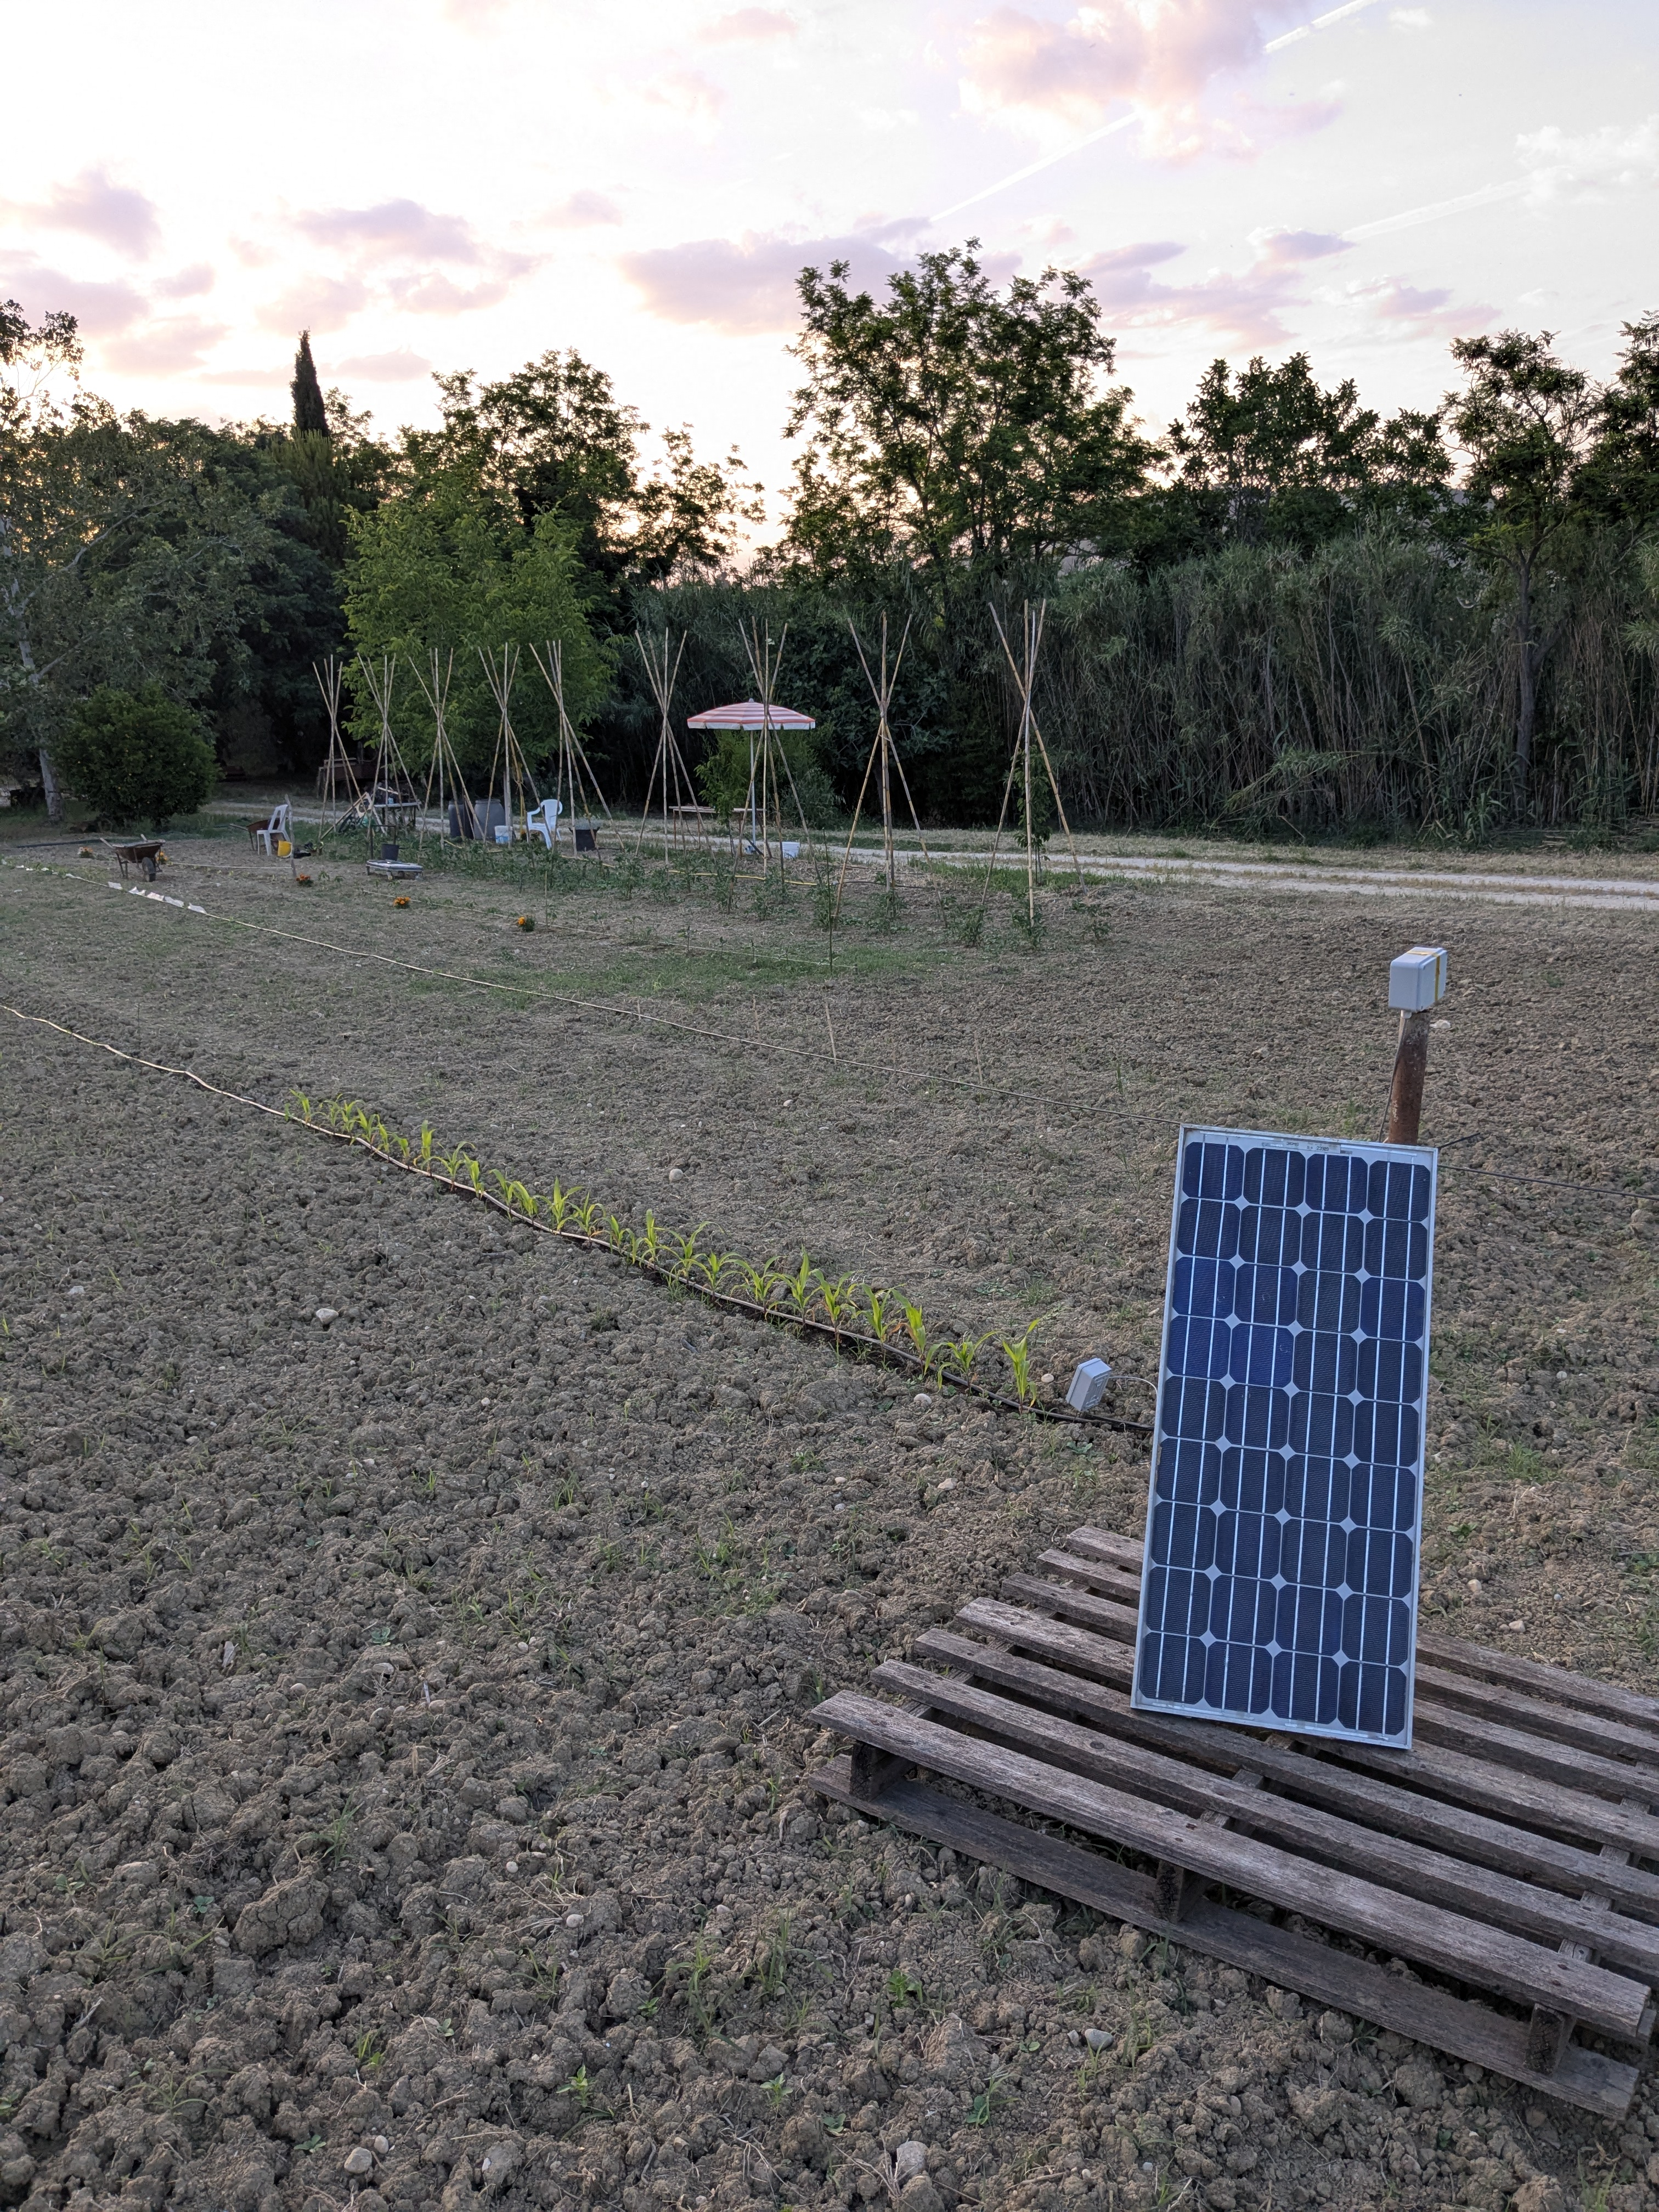
\includegraphics[width=0.4\textwidth]{media/pannello-solare-orto.jpg}
    \caption{Foto del pannello fotovoltaico utilizzato per alimentare il microcontrollore}
    \label{fig:pannello-fotovoltaico}

\end{figure}
Una volta appoggiato su di un palo conficcato nel terreno, basta collegare il pannello alle batterie.
È consigliabile interporre tra i poli del modulo fotovoltaico e le batterie un regolatore di carica, che permette
di evitare sovraccarichi e scariche profonde delle batterie, che potrebbero danneggiarle.
Nel mio caso ho optato per un covertitore DC-DC con ingresso fino a 50 V un'uscita regolabile che ho impostato a 8,2 V,
che è la tensione di carica delle due batterie 18650 collegate in serie.

\subsubsection{\terzaFaseHA}
Per una corretta misurazione dell'umidità del terreno, è necessario posizionare il sensore in modo che
la terra sotto di esso sia influenzata dall'irrigazione a goccia e che sia raggiungibile dalla rete Wi-Fi.
\begin{figure}[H]

    \centering
    \includegraphics[width=0.4\textwidth]{media/posizionamento-sensore-umidità.jpg}
    \caption{Foto del sensore di umidità posizionato all'interno dell'orto}
    \label{fig:sensore-umidita-posizionato}

\end{figure}
Per quanto riguarda il posizionamento dello switch, è sufficiante che esso si trovi in prossimità
della presa di corrente a cui è collegata la pompa e che, ovviamente, sia raggiungo dalla rete Wi-Fi.

\subsubsection{\quartaFaseHA}
Le automazioni necessarie per prendere il sistema indipendente sono le seguenti:
\begin{itemize}
    \item Accensione della pompa quando il sensore di umidità legge un valore inferiore al 75\% e quando l'orario
          è compreso tra le 22:30 e le 23:30;
    \item Spegnimento della pompa quando il sensore di umidità legge un valore superiore al 85\% e quando l'orario
          è compreso tra le 22:30 e le 23:30;;
    \item Accensione della pompa quando viene premuto il pulsante fisico di accensione;
    \item Spegnimento della pompa quando viene premuto il pulsante fisico di spegnimento.
\end{itemize}
\begin{figure}[H]
    
    \centering
    \includegraphics[width=1\textwidth]{media/screen-automazioni-homeassistant.png}
    \caption{Screenshot del menù delle automazioni di Home Assistant}
    \label{fig:automazioni-home-assistant}

\end{figure}
Tutto ciò è possibile attraverso lo strumento automazioni nelle impostazioni di Home Assistant, grazie ad
un'interfaccia grafica che permette di creare regole personalizzate.

\subsubsection{\quintaFaseHA}

La configurazione della dashboard di Home Assistant è un passaggio fondamentale per la corretta visualizzazione
dei dati raccolti e l'interazione con gli switch e i sensori.
Ciò è possibile attraverso lo strumento grafico di personalizzazione della dashboard, al quale si accede
dal menu principale tramite l'icona della matita. Questo strumento permette di selezionare quali entità
mostrare, personalizzarne l'aspetto e organizzare le informazioni in base alla prioprità che
si desidera assegnare a ciascuna di esse.

\section{Risultato}
Il lato affascinante di questo progetto è che, essendo artigianale e personale, non presenta
un punto di arrivo, ma è piuttosto un processo in continua evoluzione. Le obiettivi (milestones) raggiunti finora
hanno permesso di creare un sistema di irrigazione automatica, come specificato negli obiettivi,
ma nulla toglie che in futuro si possano integrare numerose nuove funzionalità, come ad esempio:
\begin{itemize}
    \item L'integrazione di sensori nel pollaio per monitorare le condizioni ambientali e lo stato delle galline;
    \item Apertura e chiusura automatica del pollaio in base all'orario del tramonto e dell'alba;
    \item Gestione remota del cancello di casa tramite Home Assistant;
    \item Integrazione di un sistema di sorveglianza.
    \item Integrazione di un sistema di monitoraggio della temperatura e del vento nell'orto 
            per prevedere la durata dell'irrigazione;
    \item Integrazione di una \textit{API}\footnote{Un'API, Application Programming Interface, 
            è un insieme di regole e protocolli che consente a diverse applicazioni software di comunicare tra loro.}
            per la consultazione del meteo e regolare l'irrigazione in base alle previsioni;
\end{itemize}
Dopo varie considerazioni, ho ritenuto opportuno limitare l'irrigazione solamente
alle ore notturne per facilitare l'assorbimento dell'acqua da parte delle piante e per evitarne
l'evaporazione durante le ore più calde della giornata.
Ad oggi, il sistema è completamente autonomo: ogni notte, in caso l'umidità percepita dal sensore
sia sotto il valore menimo, la pompa del pozzo si accende automaticamente e irriga le piante
fino a quando il sensore non legge un valore di umidità superiore a quello massimo stabilito.

\begin{figure}
    
    \centering
    \includegraphics[width=1\textwidth]{media/dashboard-home-assistant.png}
    \caption{Screenshot della dashboard di Home Assistant}
    \label{fig:dashboard-home-assistant}

\end{figure}

\section{Osservazioni e riflessioni}

Questo progetto, anche nella forma attuale, offre potenzialità che vanno oltre la semplice automazione dell'irrigazione.
Home Assistant offre nativamente un servizio di \textit{data logging}, che permette di registrare i dati raccolti dai 
sensori e di analizzarli nel tempo. Permette di visualizzare grafici e statistiche generati dinamicamente,
che possono essere utili per comprendere le tendenze e i modelli di crescita delle piante e per ottimizzare
le pratiche di irrigazione futuri.\\
\\
Nulla vieta l'implementazione di un sistema basato su AI e
Machine Learning\footnote{Il Machine Learning è un insieme di 
tecniche che permettono ai computer di apprendere dai dati e migliorare le proprie prestazioni senza 
essere esplicitamente programmati.} per modificare
i treshold (le soglie) di umidità in base all'andamento dei dati raccolti per migliorare l'efficienza del sistema.
Inoltre, la possibilità di integrare altri sensori e dispositivi in futuro rende fruibili nuove informazioni,
come la temperatura del terreno, il vento e le condizioni meteorologiche, permette di creare un modello predittivo
ancora più accurato. Ovviamente per permettere ciò sarà necessaria l'implementazione di una 
database\footnote{Un database è un sistema organizzato per la raccolta,
memorizzazione e gestione di dati,} relazionale,
che permetta di memorizzare, ordinare ed elaborare i dati raccolti.

\section{Conclusioni}

Il progetto \textbf{"Simone Home Hub"} ha dimostrato con successo come 
l'integrazione di tecnologie \textbf{IoT} e piattaforme \textit{open-source} come \textbf{Home Assistant} 
ed \textbf{ESPHome} possa rivoluzionare la gestione della nostra abitazione e, in questo 
caso specifico, del nostro orto. Partendo da un'esigenza concreta, l'\textbf{automazione 
dell'irrigazione} per alleviare un compito ripetitivo, siamo riusciti a 
implementare un sistema \textbf{robusto}, \textbf{efficiente} e completamente \textbf{autonomo}.

L'adozione di Home Assistant come fulcro del sistema si è rivelata una scelta vincente, 
soprattutto per la sua filosofia 
\textit{local-first}\footnote{La filosofia \textit{local-first} implica che le operazioni e i processi
siano eseguiti principalmente sul dispositivo locale, piuttosto che su server remoti
o cloud. Questo approccio garantisce maggiore affidabilità, velocità di risposta e privacy dei dati.}
. Questo approccio non solo garantisce maggiore 
\textbf{affidabilità} e \textbf{rapidità} nella risposta, non dipendendo da servizi cloud esterni e connessioni 
internet, ma pone anche un'enfasi cruciale sulla \textbf{privacy} dei dati. In un'era in cui la raccolta 
e l'analisi delle informazioni personali sono sempre più pervasive, avere il pieno controllo sui 
dati generati dalla propria casa intelligente è un valore aggiunto inestimabile. La natura \textit{DIY} 
di Home Assistant ed ESPHome, sebbene richieda un investimento iniziale di 
tempo e apprendimento, ripaga ampiamente in termini di \textbf{personalizzazione} e comprensione profonda 
del sistema che si sta costruendo. Ogni componente, dal microcontrollore al sensore, è 
configurato e programmato con precisione, consentendo un adattamento su misura alle esigenze 
specifiche dell'utente, molto più di quanto sia possibile con soluzioni \textit{"chiavi in mano"} proprietarie.

La realizzazione dell'infrastruttura di rete, con l'installazione e configurazione dell'access point, 
ha rappresentato un passo fondamentale per estendere la connettività Wi-Fi fino all'orto, creando 
l'ambiente ideale per la comunicazione dei dispositivi IoT. La scelta di \textbf{riutilizzare} hardware datato 
per il server di Home Assistant e per il pannello fotovoltaico, oltre a essere una soluzione economicamente 
vantaggiosa, è un esempio di \textbf{economia circolare} applicata alla tecnologia, riducendo gli sprechi e dando nuova vita a 
dispositivi altrimenti destinati al disuso.

\begin{figure}[H]
    \centering
    \includegraphics[width=1\textwidth]{media/dashboard-home-assistant-grafico.png}
    \caption{Grafico dell'umidità del terreno nel tempo, generato da Home Assistant}
    \label{fig:grafico-umidita}
\end{figure}

Il cuore pulsante del progetto, l'\textbf{automazione dell'irrigazione}, è stato implementato 
con successo grazie all'uso di \textbf{ESPHome}. La capacità di creare firmware 
personalizzati tramite file \texttt{YAML}, rendendo la programmazione accessibile anche a 
chi non ha profonde conoscenze di codice, ha semplificato enormemente lo sviluppo. 
La calibrazione precisa del sensore di umidità e l'integrazione di interruttori 
fisici per un controllo manuale hanno garantito \textbf{flessibilità} e \textbf{affidabilità}. L'alimentazione autonoma tramite 
pannello fotovoltaico, infine, ha eliminato la necessità di una connessione alla rete elettrica, rendendo il 
sistema \textbf{indipendente} e \textbf{sicuro}, un aspetto non trascurabile considerando il contesto agricolo.
I risultati ottenuti sono tangibili: il sistema di irrigazione ora si attiva autonomamente, ottimizzando il 
consumo idrico e garantendo un'irrigazione mirata in base alle reali necessità del terreno, specialmente 
nelle ore più fresche della giornata (\textit{nelle ore notturne}) per massimizzare l'assorbimento ed evitare l'evaporazione. Questo non 
solo libera tempo prezioso per me, mio padre e mio zio, ma contribuisce anche a una gestione più \textbf{sostenibile} 
delle risorse idriche.\\
\\
Questo progetto, tuttavia, non è un punto di arrivo, ma piuttosto un \textbf{trampolino di lancio} per ulteriori sviluppi.
Le \textbf{potenzialità} dell'IoT e di Home Assistant sono pressoché illimitate. Le future implementazioni, come il 
monitoraggio del pollaio, l'automazione dell'apertura/chiusura o la gestione remota del cancello, sono solo 
alcune delle direzioni che si potrebbero intraprendere. Ogni nuova integrazione non solo accresce il comfort 
abitativo, ma offre anche nuove opportunità di raccolta dati.
A tal proposito, le osservazioni sui dati meritano una riflessione più profonda. Home Assistant, con le sue 
capacità di \textbf{data logging}, ci fornisce un \textbf{tesoro} di informazioni. L'analisi dei trend di umidità del terreno, 
correlati alle condizioni climatiche e alle abitudini di irrigazione, può portare a una comprensione senza 
precedenti dei bisogni delle nostre piante. Si potrebbe immaginare un futuro in cui un sistema basato su 
\textbf{intelligenza artificiale} analizzi questi dati per ottimizzare dinamicamente le soglie di irrigazione, 
adattandosi ai cambiamenti stagionali o a eventi meteorologici imprevisti, portando l'efficienza a un 
livello superiore.\\
\\
Quanto sopra ci invita a riflettere su come i dati, se ben gestiti e analizzati, possano 
non solo automatizzare, ma anche \textbf{ottimizzare} e \textbf{migliorare} le nostre pratiche quotidiane, rendendo le 
nostre case non solo "\textbf{smart}", ma anche più "\textbf{consapevoli}" e "\textbf{resilienti}", aiutando anche noi a diventarlo.
In definitiva, il progetto \textbf{"Simone Home Hub"} è un esempio lampante di come la tecnologia, se 
applicata con intelligenza e visione, possa migliorare significativamente la qualità della vita, 
rendendo i nostri ambienti più \textbf{efficienti}, \textbf{sicuri} e, in ultima analisi, più \textbf{intelligenti}. È un invito a 
\textbf{esplorare}, \textbf{sperimentare} e \textbf{costruire}, dimostrando che il futuro delle nostre case è nelle nostre mani.
\vfill
\begin{figure}[H]
    \centering
    \includegraphics[width=0.2\textwidth]{media/qr-code.png}
    \caption{Qr code per accedere al repository GitHub del progetto}
    \label{fig:simone-home-hub-qr-code}
\end{figure}
\vfill


\end{document}